% !TEX root=./../maha-dip-notes.tex
\chapter{Binary Image Processing}

\section{Introduction}

\dfn{Image Definition}{
An \textbf{image} is a projection of a 3D object onto a 2D surface. This dimensional reduction causes loss of certain 3D information, which is generally very hard to recover. 
}


\section{Image Formation}

The process of \textbf{image formation} models how a 3D scene is mapped to a 2D image plane through a camera model. A pinhole camera serves as the simplest abstraction to study this process.

\subsection{Pinhole Camera Model (2D)}
In the 2D case, the relation between a point $(X,Z)$ in the scene and its projection $(x)$ on the image plane is derived by similar triangles:

\vspace{1cm}


\begin{center}
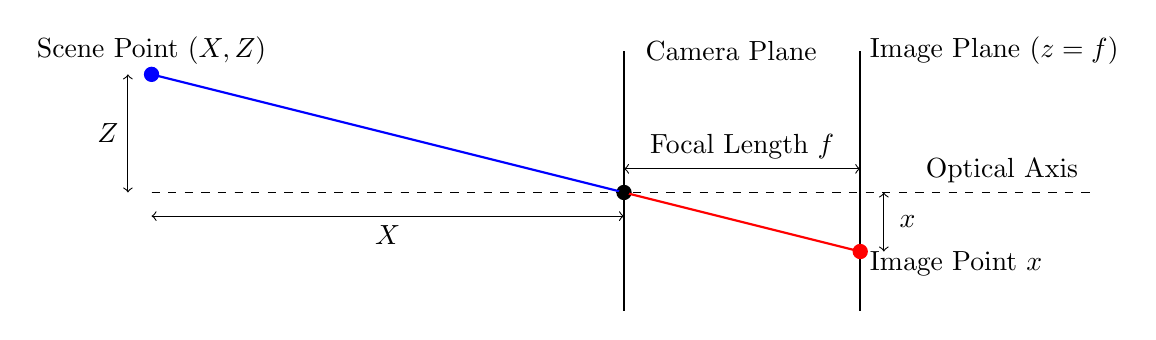
\begin{tikzpicture}[scale=1.5]
  % Draw the image plane
  \draw[thick] (6,0) -- (6,2.2);
  \node[right] at (6,2.2) {Image Plane ($z=f$)};
  % Draw the image plane
  \draw[thick] (4,0) -- (4,2.2);
  \node[right] at (4.1,2.2) {Camera Plane};
  % Draw the optical axis
  \draw[dashed] (0,1) -- (8,1);
  \node[above] at (7.2,1) {Optical Axis};
  % Draw the pinhole (center of projection)
  \filldraw[black] (4,1) circle (0.06);
  % \node[above] at (4.6,0.6) {Pinhole $O$};
  % Draw the scene point (object) on the left
  \filldraw[blue] (0,2) circle (0.06);
  \node[above] at (0,2) {Scene Point $(X,Z)$};
  % Draw projection line from scene point to pinhole
  \draw[blue,thick] (0,2) -- (4,1);
  % Draw projection line from pinhole to image plane (right side)
  \draw[red,thick] (4,1) -- (6,0.5);
  % Draw the projected point on image plane
  \filldraw[red] (6,0.5) circle (0.06);
  \node[right] at (6,0.4) {Image Point $x$};
  % Label distances
  \draw[<->] (0,0.8) -- (4,0.8);
  \node[below] at (2,0.8) {$X$};
  \draw[<->] (-0.2,1) -- (-0.2,2);
  \node[left] at (-0.2,1.5) {$Z$};
  \draw[<->] (6.2,1) -- (6.2,0.5);
  \node[right] at (6.25,0.75) {$x$};
  \draw[<->] (6,1.2) -- (4,1.2);
  \node[above] at (5,1.2) {Focal Length $f$};
  % Draw focal length line
  \draw[dashed] (0,1) -- (4,1);
  \filldraw[black] (4,1) circle (0.04);
\end{tikzpicture}
\end{center}

\vspace{0.3cm}

\noindent from the diagram, we have:

\[
\frac{x}{f} = \frac{X}{Z}
\quad \Rightarrow \quad
x = f \cdot \frac{X}{Z}
\]
Here, $f$ is the focal length of the pinhole camera.


\nt{we use Capital letters for 3D coordinates and lowercase for 2D image coordinates and observe that the \textrm{Z} component is lost.}

\subsection{Pinhole Camera Model (3D)}
Extending to 3D coordinates $(X,Y,Z)$, the projection onto the image plane gives:
\[
x = f \cdot \frac{X}{Z}, \quad
y = f \cdot \frac{Y}{Z}
\]

\noindent This shows how 3D geometry is mapped to 2D via perspective projection.

\subsection{Homogeneous Coordinates}
Homogeneous coordinates are used to express projection as a matrix multiplication:
\[
\begin{bmatrix}x \\ y \\ 1 \end{bmatrix}
= \frac{1}{Z}
\begin{bmatrix}
f & 0 & 0 & 0 \\
0 & f & 0 & 0 \\
0 & 0 & 1 & 0
\end{bmatrix}
\begin{bmatrix} X \\ Y \\ Z \\ 1 \end{bmatrix}
\]

\nt{Homogeneous coordinates are crucial because they unify perspective projection, translation, and rotation into matrix multiplications.}

\subsection{Intrinsic Matrix}
The \textbf{intrinsic parameters} capture camera-specific properties such as focal length and principal point offset:
\[
K =
\begin{bmatrix}
f_x & 0 & c_x \\
0 & f_y & c_y \\
0 & 0 & 1
\end{bmatrix}
\]
where $(f_x,f_y)$ are focal lengths in pixel units and $(c_x,c_y)$ is the principal point.

\subsection{Extrinsic Matrix}
The \textbf{extrinsic parameters} describe the camera’s position and orientation in the world:
\[
M = [R|t]
\]
where $R$ is a $3\times 3$ rotation matrix and $t$ is a $3 \times 1$ translation vector.

\nt{
The rotation matrix $R$ can be defined using an angle $\alpha$ in 2D as:
\[
R(\alpha) = 
\begin{bmatrix}
\cos\alpha & -\sin\alpha \\
\sin\alpha & \cos\alpha
\end{bmatrix}
\]
This matrix rotates a point by $\alpha$ radians in the plane.
% }
% \nt{
In 3D, rotation can be performed about each axis using three matrices:
\[
R_x(\theta) = 
\begin{bmatrix}
1 & 0 & 0 \\
0 & \cos\theta & -\sin\theta \\
0 & \sin\theta & \cos\theta
\end{bmatrix}
% \]
% \[
\quad , \quad
R_y(\phi) = 
\begin{bmatrix}
\cos\phi & 0 & \sin\phi \\
0 & 1 & 0 \\
-\sin\phi & 0 & \cos\phi
\end{bmatrix}
% \]
% \[
\quad , \quad
R_z(\psi) = 
\begin{bmatrix}
\cos\psi & -\sin\psi & 0 \\
\sin\psi & \cos\psi & 0 \\
0 & 0 & 1
\end{bmatrix}
\]
A general 3D rotation can be represented by multiplying these matrices:
\[
R = R_z(\psi) R_y(\phi) R_x(\theta)
\]
where $\theta$, $\phi$, and $\psi$ are rotation angles about the $x$, $y$, and $z$ axes, respectively.

}

\subsection{Projection Matrix}
The complete mapping from 3D world coordinates to 2D image plane is:
\[
s \begin{bmatrix} u \\ v \\ 1 \end{bmatrix}
= K M 
\begin{bmatrix} X \\ Y \\ Z \\ 1 \end{bmatrix}
\]
with scaling factor $s$.  

\clm{Projection Matrix}{}
{The projection matrix $P = K @ M$ completely defines the mapping from world coordinates to image coordinates, which depends on the intrinsic and extrinsic parameters of the camera. (i.e., focal length, principal point, rotation, and translation vectors.)}

% \subsection{Camera Calibration}
\dfn{Camera Calibration}{The process of estimating the intrinsic and extrinsic parameters of a camera from observed images of a known calibration pattern.}
Calibration ensures accurate geometric measurements from images.


\section{Image Representation}

\subsection{Pixel Values}
A digital image is represented as a 2D array of \textbf{pixels (picture elements)}, each encoding intensity (grayscale) or color.


\dfn{Image \& Pixel}{%
An \textbf{image} is a 2D array $$I:\{0,\dots,M-1\}\times\{0,\dots,N-1\}\to\{0,\dots,K-1\}$$
Each element $I[i,j]$ is a \textbf{pixel} with \textbf{intensity} (gray level) in $\{0,\dots,K-1\}$, where, 0 represents black and $K-1$ represents white. For a 8 bit storage, $B = 8$, then maximum intensity can be calculated as $K = 2^B = 2^8 = 256$, $0$ represents black and $255$ represents white. \\

For normalized intensity, use $$I_n[i,j]=\frac{I[i,j]}{(K-1)}\in[0,1]$$.%
}

\subsection{Color Spaces}
Different \textbf{color spaces} represent pixel values differently:
\begin{itemize}
    \item RGB: additive primary colors.
    \item HSV: hue, saturation, value (closer to human perception).
    \item YCbCr: luminance and chrominance separation. (where Y is intensity)
\end{itemize}



\subsection{Feature Extraction and Descriptors}
\textbf{Features} capture essential information in images such as edges, corners, or textures.  
\textbf{Descriptors} encode features into numerical representations (e.g., SIFT, HOG) for matching and recognition.

\subsection{Sampling and Quantization}
The ideal irradiance signal is sampled on a discrete grid and quantized to a finite set of gray levels.
\begin{itemize}
    \item \textbf{Sampling:} Selecting discrete spatial points to represent an image.\\
    choose integer pixel sites $(i,j)$; the image becomes $I[i,j]$ on an $M\times N$ grid.
    \item \textbf{Quantization:} Mapping continuous intensity values into discrete levels \\
    map real intensities to $\{0,1,\dots,K-1\}$, e.g., $K=256$ for 8-bit grayscale.
\end{itemize}

\noindent \textbf{Binary images:} special case $K=2$ with intensities $\{0,1\}$ (or $\{0,255\}$ in 8-bit storage).



\nt{Undersampling causes aliasing; inadequate quantization leads to loss of detail.}

\subsection{Image Formats}
Typical resolutions include $256\times 256$, $512\times 512$, \textbf{1920x1080}, etc.%
As we can calculate the number of Bytes required to store these images, we find:

\begin{itemize}
    \item For $256\times 256$ images: $256 \times 256 \times 1 = 65,536$ Bytes (assuming 8-bit grayscale).
    \item For $512\times 512$ images: $512 \times 512 \times 1 = 262,144$ Bytes (assuming 8-bit grayscale).
    \item For $1920\times 1080$ images: $1920 \times 1080 \times 3 = 6,220,800$ Bytes (assuming 24-bit RGB).
\end{itemize}

which is nearly 6.3 MB for a full HD image (1920x1080 3-channel RGB image). 
Hence, image storage can be quite substantial, necessitating efficient compression techniques. \\

Few common \textbf{Formats} include:
\begin{itemize}
    \item JPEG: lossy compressed format. \\
    The most common for photographs to save space, as the human eye is less sensitive to high-frequency details. The compression is achieved by discarding some image data, but the benefit is a significantly reduced file size. (e.g. the full HD image (1920x1080) can be compressed from {\bf 6.3 MB} to around less than a {\bf 1 MB})
    \item PNG: lossless compression, supports transparency.
    \item BMP: uncompressed raster format.
    \item TIFF: flexible format supporting various compressions.
    \item GIF: supports animation and transparency (limited color palette).
    \item WEBP: modern format providing lossy and lossless compression.
    \item HEIF: high efficiency image format, supports advanced features.
    \item AVIF: image format based on AV1 compression, offering high quality at smaller file sizes.
    \item EXR: high dynamic range (HDR) image format, supports wide color gamuts and high bit depths.
    \item DNG: raw image format for digital photography, preserves original sensor data.
    \item PPM: portable pixmap format, simple uncompressed color image format.
\end{itemize}

\subsection{Binary Images and Thresholding}

\dfn{Binary Image}{
A \textbf{binary image} is an image that consists of only two colors, typically black and white. Each pixel in a binary image is represented by a single bit, where 0 represents black and 1 represents white.
}


\noindent The simplest method to obtain binary images is \textbf{thresholding}:
\[
B(x,y) = \begin{cases}
1 & I(x,y) \geq T \\
0 & I(x,y) < T
\end{cases}
\]
where $T$ is the threshold.

\subsection{Gray Level Histograms}
The histogram of grayscale values is a fundamental tool to analyze and design thresholding algorithms.

\clm{Histogram-based Thresholding}{}
{If the histogram shows two well-separated peaks, the optimal threshold lies near the valley between them.}



%==========================
\section{Histogram of an Image}
%==========================

\dfn{Gray-Level Histogram}{
A \textbf{gray-level histogram} is a representation of the distribution of pixel intensities in a grayscale image. It counts the number of pixels for each intensity level, providing insights into the image's contrast and brightness.
}
\paragraph{Mathematical Formulation}

Let a grayscale image be
$$I:\{0,\dots,M\!-\!1\}\times\{0,\dots,N\!-\!1\}\to\{0,\dots,K\!-\!1\}$$. 
The \emph{histogram} counts occurrences at each gray level, given as a function as 
$$H:\{0,\dots,K\!-\!1\}\to\{0,\dots,MN\}$$

such that 
$$ H(k) = \text{no of occurrences of gray level } k$$ 

where $k \in \{0,\dots,K-1\}$

\[
H(k) \;=\; \#\{(i,j): I[i,j]=k\} \qquad k=0,\dots,K-1
\]

also, 
\[
\sum_{k=0}^{K-1} H(k)=MN.
\]

\noindent The \emph{normalized histogram} (PMF) is $$p(k)=\tfrac{H(k)}{MN}$$

and $$\sum_k p(k)=1$$


\ex{Interpreting Histogram Shapes}{
Given an image whose histogram exhibits a tall peak near intensity $40$ (dark shades), and another smaller, broad peak near $200$ (bright shades), we deduce the image features a dark background with a bright foreground—ideal for segmentation via thresholding.

\begin{itemize}
\item \textbf{Dark image:} $p(k)$ concentrated near $k\approx 0$.
\item \textbf{Bright image:} $p(k)$ concentrated near $k\approx K\!-\!1$.
\item \textbf{Bimodal image:} two peaks (e.g., dark foreground on bright background) $\Rightarrow$ suitable for a \emph{single} global threshold.
\end{itemize}

\begin{center}
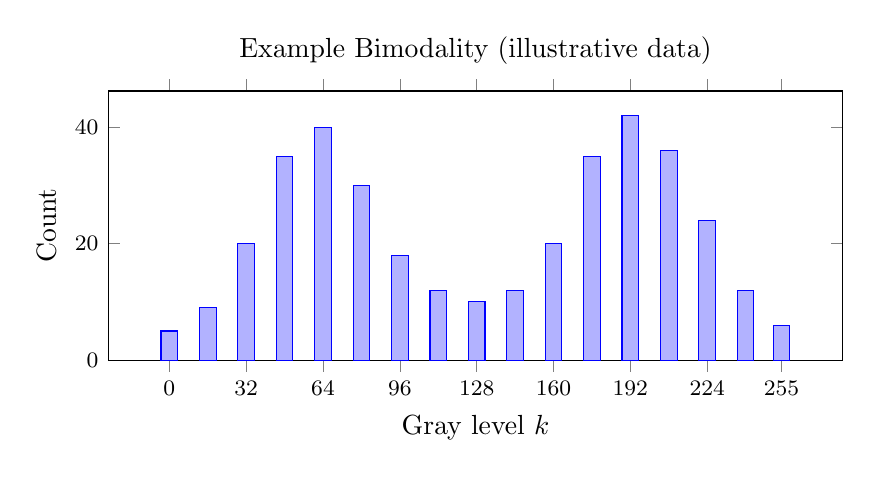
\begin{tikzpicture}
\begin{axis}[
  ybar, bar width=6pt, width=0.9\linewidth, height=5cm,
  ymin=0, ylabel={Count}, xlabel={Gray level $k$},
  xtick={0,32,64,96,128,160,192,224,255},
  xticklabel style={font=\footnotesize}, yticklabel style={font=\footnotesize},
  title={Example Bimodality (illustrative data)}
]
\addplot coordinates {(0,5) (16,9) (32,20) (48,35) (64,40) (80,30) (96,18) (112,12)
(128,10) (144,12) (160,20) (176,35) (192,42) (208,36) (224,24) (240,12) (255,6)};
\end{axis}
\end{tikzpicture}
\end{center}
}

% Gray level image histograms are foundational tools in digital image processing, providing a statistical representation of the distribution of pixel intensities in an image. The histogram constitutes an array or plot where the $x$-axis denotes possible gray levels (e.g., $0$ to $255$ for 8-bit images), and the $y$-axis gives the count or probability of each gray level's appearance within the image.

\nt{Understanding the histogram profile assists in identifying whether an image is underexposed, overexposed, well-contrasted, or subject to other illumination artifacts.}


\paragraph{Types of Histograms and Their Interpretation}
Different histogram profiles relate directly to the visual impression and underlying properties of an image:
\begin{itemize}
    \item \textbf{Bright Images:} Most pixel values clustered towards the higher end of the gray level range.
    \item \textbf{Dark Images:} Values crowded in the lower end, leading to overall darker visual output.
    \item \textbf{Dual Peak Model:} Exhibits two pronounced peaks, often corresponding to distinct foreground and background regions; common in images fit for binarization.
    \item \textbf{Flat Histogram:} Pixels uniformly distributed across gray levels—rare in natural images, may occur in images heavily corrupted with noise.
    \item \textbf{Equal Histograms:} Result from histogram equalization operations to improve contrast.
\end{itemize}

\ex{Histogram Interpretation}{
\begin{itemize}
    \item A \textbf{bright image} shows histogram concentrated on high intensity values.
    \begin{center}
      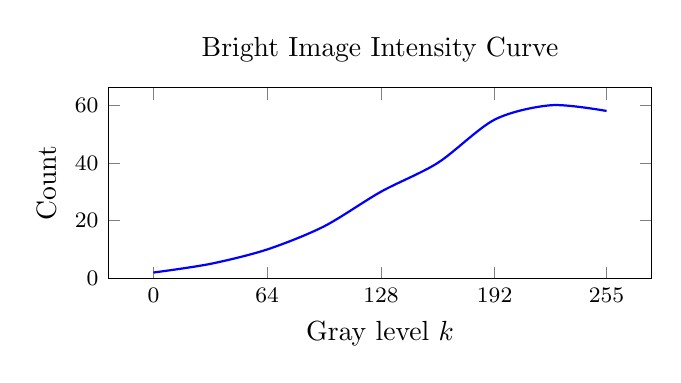
\begin{tikzpicture}
      \begin{axis}[
        width=0.7\linewidth, height=4cm,
        ymin=0, ylabel={Count}, xlabel={Gray level $k$},
        xtick={0,64,128,192,255},
        xticklabel style={font=\footnotesize}, yticklabel style={font=\footnotesize},
        title={Bright Image Intensity Curve}
      ]
      % Smooth curve through the points
      \addplot[
        smooth, thick, blue
      ] coordinates {
        (0,2) (32,5) (64,10) (96,18) (128,30) (160,40) (192,55) (224,60) (255,58)
      };
      \end{axis}
      \end{tikzpicture}
      \\
      \emph{Intensity profile of a bright image: curve shifted towards high gray levels}
    \end{center}
    \item A \textbf{dark image} shows histogram concentrated on low values.
    \begin{center}
      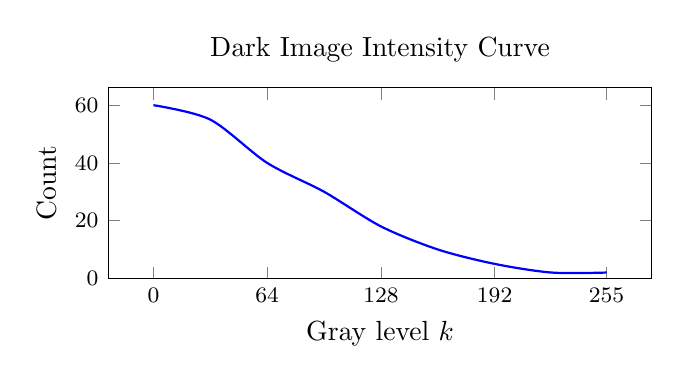
\begin{tikzpicture}
      \begin{axis}[
        width=0.7\linewidth, height=4cm,
        ymin=0, ylabel={Count}, xlabel={Gray level $k$},
        xtick={0,64,128,192,255},
        xticklabel style={font=\footnotesize}, yticklabel style={font=\footnotesize},
        title={Dark Image Intensity Curve}
      ]
      % Smooth curve through the points
      \addplot[
        smooth, thick, blue
      ] coordinates {
        (0,60) (32,55) (64,40) (96,30) (128,18) (160,10) (192,5) (224,2) (255,2)
      };
      \end{axis}
      \end{tikzpicture}
      \\
      \emph{Intensity profile of a dark image: curve shifted towards low gray levels}
    \end{center}
    \item A \textbf{dual-peak image} indicates presence of both dark (background) and bright (foreground) regions.
    \begin{center}
      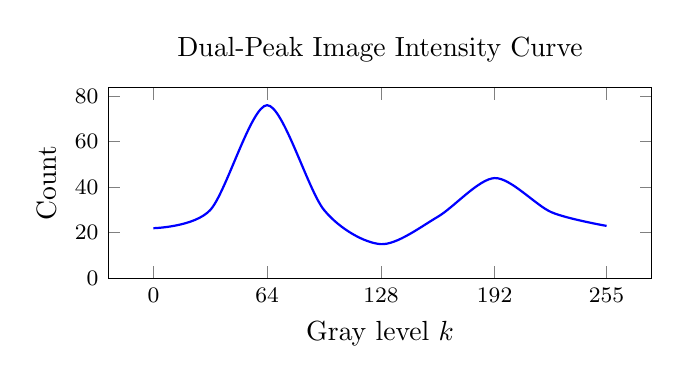
\begin{tikzpicture}
      \begin{axis}[
        width=0.7\linewidth, height=4cm,
        ymin=0, ylabel={Count}, xlabel={Gray level $k$},
        xtick={0,64,128,192,255},
        xticklabel style={font=\footnotesize}, yticklabel style={font=\footnotesize},
        title={Dual-Peak Image Intensity Curve}
      ]
      % Smooth curve through the points
      \addplot[
        smooth, thick, blue
      ] coordinates {
        (0,22) (32,30) (64,76) (96,30) (128,15) (160,27) (192,44) (224,29) (255,23)
      };
      \end{axis}
      \end{tikzpicture}
      \\
      \emph{Intensity profile of a dual-peak image: two distinct peaks at low and high gray levels}
    \end{center}

    \item A \textbf{flat histogram} corresponds to uniformly distributed intensities.
    \begin{center}
      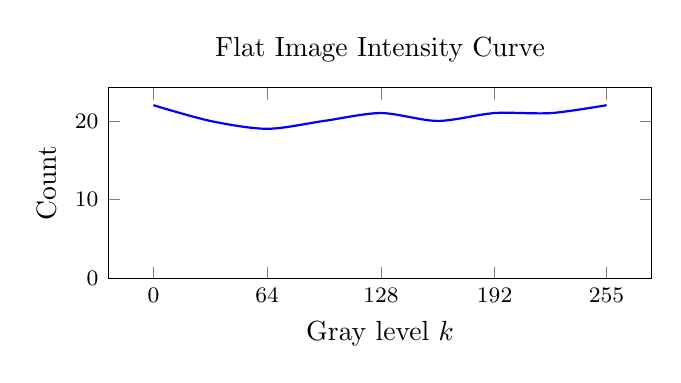
\begin{tikzpicture}
      \begin{axis}[
        width=0.7\linewidth, height=4cm,
        ymin=0, ylabel={Count}, xlabel={Gray level $k$},
        xtick={0,64,128,192,255},
        xticklabel style={font=\footnotesize}, yticklabel style={font=\footnotesize},
        title={Flat Image Intensity Curve}
      ]
      % Smooth curve through the points
      \addplot[
        smooth, thick, blue
      ] coordinates {
        (0,22) (32,20) (64,19) (96,20) (128,21) (160,20) (192,21) (224,21) (255,22)
      };
      \end{axis}
      \end{tikzpicture}
      \\
      \emph{Intensity profile of a flat image: uniform distribution across all gray levels}
    \end{center}

\end{itemize}

\textbf{At a Glance:}

\begin{center}
\renewcommand{\arraystretch}{1.2}
\begin{tabular}{@{}p{3.2cm}p{4.8cm}p{4.8cm}@{}}
\toprule
\textbf{Histogram Type} & \textbf{Typical Scene} & \textbf{Segmentation Implication} \\
\midrule
Dark-skewed & Low-light or dark objects & Threshold near lower gray levels \\
Bright-skewed & Bright background/lighting & Threshold near higher gray levels \\
Bimodal & Foreground vs.\ background & Global threshold often effective \\
Flat/noisy & Low contrast/high noise & Consider contrast stretch or adaptive threshold \\
\bottomrule
\end{tabular}
\end{center}


}


\section{Otsu's Binarization}

Otsu’s thresholding is a non-parametric, unsupervised method for automatic image binarization. It determines the optimal threshold to separate foreground and background by maximizing inter-class variance.

\subsection{Probability and Statistical Prerequisites}

\paragraph{Basic Probability Concepts}
Consider an image histogram with $L$ gray levels ($0, 1, ..., L-1$). Let $p_k$ denote the normalized probability for gray level $k$:
$$
p_k = \frac{n_k}{N}
$$
where $n_k$ is the number of pixels with gray level $k$, and $N$ is the total pixel count.

\subsubsection{Class Probabilities, Means, and Variances}
For a given threshold $T$:

\noindent \textbf{Class Probability}
\begin{itemize}
\item Probability that the pixel belongs to class 0 (background)
\[
\omega_0(T) = \sum_{k=0}^T p _k \quad\text{(Probability of class 0 - background - black pixels)}
\]
\item Probability that the pixel belongs to class 1 (foreground)
\[\omega_1(T) = \sum_{k=T+1}^{L-1} p_k \quad\text{(Probability of class 1 - foreground - white pixels)} 
\]
\end{itemize}

\noindent \textbf{Class Means} 
\begin{itemize}
  

\item  Probability that the pixel takes values k given that it belongs to class 0
\begin{align*}
\mu_0(T) &= \sum_{k=0}^T k \cdot p(k | C_0)  \quad\text{(Mean of class 0)} \\
\text{where} \quad p(k | C_0) &= \frac{p(k, C_0)}{p(C_0)} = \frac{p_k p(C_0 | k)}{p(C_0)} \\
\text{for} k \in \{ 0\dots T \} \quad p(k | C_0) &= \frac{p_k}{\omega_0(T)} \\
\mu_0(T) &=\frac{1}{\omega_0(T)} \sum_{k=0}^T k p_k \\
\text{also, for} k \in \{ T+1 \dots L-1 \} \quad p(k | C_0) &= 0\\ 
\mu_0(T) &=\frac{1}{\omega_0(T)} \sum_{k=0}^{L-1} k p_k
\end{align*}
\item Probability that the pixel takes values k given that it belongs to class 1
\begin{align*}
\mu_1(T) &= \sum_{k=T+1}^{L-1} k \cdot p(k | C_1)  \quad\text{(Mean of class 1)} \\
\text{where} \quad p(k | C_1) &= \frac{p(k, C_1)}{p(C_1)} = \frac{p_k p(C_1 | k)}{p(C_1)} \\
\text{for} k \in \{ T+1 \dots L-1 \} \quad p(k | C_1) &= \frac{p_k}{\omega_1(T)} \\
\mu_1(T) &=\frac{1}{\omega_1(T)} \sum_{k=T+1}^{L-1} k p_k \\
\text{also, for} k \in \{ 0 \dots T \} \quad p(k | C_1) &= 0\\
\mu_1(T) &=\frac{1}{\omega_1(T)} \sum_{k=0}^{L-1} k p_k
\end{align*}

\item Overall Image Mean
\begin{align*}
\mu_T &= \sum_{k=0}^{L-1} k p_k \\
&= \sum_{k=0}^{T} k p_k + \sum_{k=T+1}^{L-1} k p_k\\ 
&= \mu_0(T) \omega_0(T) + \mu_1(T) \omega_1(T)
\end{align*}
\end{itemize}

\noindent \textbf{Class Variances}\\
\begin{itemize}
\item Variance of class 0
\begin{align*}
\sigma_0^2(T) &= \sum_{k=0}^{T} (k - \mu_0(T))^2 p(k | C_0)\\
&= \sum_{k=0}^{T} (k - \mu_0(T))^2 \frac{p_k}{\omega_0(T)}
\end{align*}

\item Variance of class 1
\begin{align*}
\sigma_1^2(T) &= \sum_{k=T+1}^{L-1} (k - \mu_1(T))^2 p(k | C_1)\\
&= \sum_{k=T+1}^{L-1} (k - \mu_1(T))^2 \frac{p_k}{\omega_1(T)}
\end{align*}

\item Total Image Variance
\begin{align*}
  \sigma^2 (T) &= \sum_{k=0}^{L-1} (k - \mu_T)^2 p_k \\
  &= \sum_{k=0}^{T} (k - \mu_T)^2 p_k + \sum_{k=T+1}^{L-1} (k - \mu_T)^2 p_k \\
  &= \sigma_0^2(T) + \sigma_1^2(T) + \omega_0(T)[\mu_0(T) - \mu_T]^2 + \omega_1(T)[\mu_1(T) - \mu_T]^2
\end{align*}
\end{itemize}

\subsection{Otsu’s Binarization: Statement and Algorithm}

\dfn{Otsu’s Binarization}{The process of determining the threshold $T^*$ that maximizes the inter-class variance between foreground and background, thus optimally segmenting a bimodal histogram image.}
